\documentclass[11pt]{article}

\usepackage{fullpage}
\usepackage{amsmath, amssymb, bm, cite, epsfig, psfrag}
\usepackage{graphicx}
\usepackage{float}
\usepackage{amsthm}
\usepackage{amsfonts}
\usepackage{listings}
\usepackage{cite}
\usepackage{hyperref}
\usepackage{tikz}
\usepackage{enumerate}
\usepackage{listings}
\usepackage{mathtools}
\usepackage{bbm}
\usepackage{array}
\lstloadlanguages{Python}
\usetikzlibrary{shapes,arrows}
%\usetikzlibrary{dsp,chains}

\DeclareFixedFont{\ttb}{T1}{txtt}{bx}{n}{9} % for bold
\DeclareFixedFont{\ttm}{T1}{txtt}{m}{n}{9}  % for normal
% Defining colors
\usepackage{color}
\definecolor{deepblue}{rgb}{0,0,0.5}
\definecolor{deepred}{rgb}{0.6,0,0}
\definecolor{deepgreen}{rgb}{0,0.5,0}
\definecolor{backcolour}{rgb}{0.95,0.95,0.92}

%\restylefloat{figure}
%\theoremstyle{plain}      \newtheorem{theorem}{Theorem}
%\theoremstyle{definition} \newtheorem{definition}{Definition}

\def\del{\partial}
\def\ds{\displaystyle}
\def\ts{\textstyle}
\def\beq{\begin{equation}}
\def\eeq{\end{equation}}
\def\beqa{\begin{eqnarray}}
\def\eeqa{\end{eqnarray}}
\def\beqan{\begin{eqnarray*}}
\def\eeqan{\end{eqnarray*}}
\def\nn{\nonumber}
\def\binomial{\mathop{\mathrm{binomial}}}
\def\half{{\ts\frac{1}{2}}}
\def\Half{{\frac{1}{2}}}
\def\N{{\mathbb{N}}}
\def\Z{{\mathbb{Z}}}
\def\Q{{\mathbb{Q}}}
\def\R{{\mathbb{R}}}
\def\C{{\mathbb{C}}}
\def\argmin{\mathop{\mathrm{arg\,min}}}
\def\argmax{\mathop{\mathrm{arg\,max}}}
%\def\span{\mathop{\mathrm{span}}}
\def\diag{\mathop{\mathrm{diag}}}
\def\x{\times}
\def\limn{\lim_{n \rightarrow \infty}}
\def\liminfn{\liminf_{n \rightarrow \infty}}
\def\limsupn{\limsup_{n \rightarrow \infty}}
\def\MID{\,|\,}
\def\MIDD{\,;\,}
\newcommand{\specialcell}[2][c]{%
  \begin{tabular}[#1]{@{}c@{}}#2\end{tabular}}

\newtheorem{proposition}{Proposition}
\newtheorem{definition}{Definition}
\newtheorem{theorem}{Theorem}
\newtheorem{lemma}{Lemma}
\newtheorem{corollary}{Corollary}
\newtheorem{assumption}{Assumption}
\newtheorem{claim}{Claim}
\def\qed{\mbox{} \hfill $\Box$}
\setlength{\unitlength}{1mm}

\def\bhat{\widehat{b}}
\def\ehat{\widehat{e}}
\def\phat{\widehat{p}}
\def\qhat{\widehat{q}}
\def\rhat{\widehat{r}}
\def\shat{\widehat{s}}
\def\uhat{\widehat{u}}
\def\ubar{\overline{u}}
\def\vhat{\widehat{v}}
\def\xhat{\widehat{x}}
\def\xbar{\overline{x}}
\def\zhat{\widehat{z}}
\def\zbar{\overline{z}}
\def\la{\leftarrow}
\def\ra{\rightarrow}
\def\MSE{\mbox{\small \sffamily MSE}}
\def\SNR{\mbox{\small \sffamily SNR}}
\def\SINR{\mbox{\small \sffamily SINR}}
\def\arr{\rightarrow}
\def\Exp{\mathbb{E}}
\def\var{\mbox{var}}
\def\Tr{\mbox{Tr}}
\def\tm1{t\! - \! 1}
\def\tp1{t\! + \! 1}
\def\Tm1{T\! - \! 1}
\def\Tp1{T\! + \! 1}


\def\Xset{{\cal X}}

\newcommand{\one}{\mathbf{1}}
\newcommand{\abf}{\mathbf{a}}
\newcommand{\bbf}{\mathbf{b}}
\newcommand{\dbf}{\mathbf{d}}
\newcommand{\ebf}{\mathbf{e}}
\newcommand{\gbf}{\mathbf{g}}
\newcommand{\hbf}{\mathbf{h}}
\newcommand{\pbf}{\mathbf{p}}
\newcommand{\pbfhat}{\widehat{\mathbf{p}}}
\newcommand{\qbf}{\mathbf{q}}
\newcommand{\qbfhat}{\widehat{\mathbf{q}}}
\newcommand{\rbf}{\mathbf{r}}
\newcommand{\rbfhat}{\widehat{\mathbf{r}}}
\newcommand{\sbf}{\mathbf{s}}
\newcommand{\sbfhat}{\widehat{\mathbf{s}}}
\newcommand{\ubf}{\mathbf{u}}
\newcommand{\ubfhat}{\widehat{\mathbf{u}}}
\newcommand{\utildebf}{\tilde{\mathbf{u}}}
\newcommand{\vbf}{\mathbf{v}}
\newcommand{\vbfhat}{\widehat{\mathbf{v}}}
\newcommand{\wbf}{\mathbf{w}}
\newcommand{\wbfhat}{\widehat{\mathbf{w}}}
\newcommand{\xbf}{\mathbf{x}}
\newcommand{\xbfhat}{\widehat{\mathbf{x}}}
\newcommand{\xbfbar}{\overline{\mathbf{x}}}
\newcommand{\ybf}{\mathbf{y}}
\newcommand{\zbf}{\mathbf{z}}
\newcommand{\zbfbar}{\overline{\mathbf{z}}}
\newcommand{\zbfhat}{\widehat{\mathbf{z}}}
\newcommand{\Ahat}{\widehat{A}}
\newcommand{\Abf}{\mathbf{A}}
\newcommand{\Bbf}{\mathbf{B}}
\newcommand{\Cbf}{\mathbf{C}}
\newcommand{\Bbfhat}{\widehat{\mathbf{B}}}
\newcommand{\Dbf}{\mathbf{D}}
\newcommand{\Gbf}{\mathbf{G}}
\newcommand{\Hbf}{\mathbf{H}}
\newcommand{\Ibf}{\mathbf{I}}
\newcommand{\Kbf}{\mathbf{K}}
\newcommand{\Pbf}{\mathbf{P}}
\newcommand{\Phat}{\widehat{P}}
\newcommand{\Qbf}{\mathbf{Q}}
\newcommand{\Rbf}{\mathbf{R}}
\newcommand{\Rhat}{\widehat{R}}
\newcommand{\Sbf}{\mathbf{S}}
\newcommand{\Ubf}{\mathbf{U}}
\newcommand{\Vbf}{\mathbf{V}}
\newcommand{\Wbf}{\mathbf{W}}
\newcommand{\Xhat}{\widehat{X}}
\newcommand{\Xbf}{\mathbf{X}}
\newcommand{\Ybf}{\mathbf{Y}}
\newcommand{\Zbf}{\mathbf{Z}}
\newcommand{\Zhat}{\widehat{Z}}
\newcommand{\Zbfhat}{\widehat{\mathbf{Z}}}
\def\alphabf{{\boldsymbol \alpha}}
\def\betabf{{\boldsymbol \beta}}
\def\betabfhat{{\widehat{\bm{\beta}}}}
\def\epsilonbf{{\boldsymbol \epsilon}}
\def\mubf{{\boldsymbol \mu}}
\def\lambdabf{{\boldsymbol \lambda}}
\def\etabf{{\boldsymbol \eta}}
\def\xibf{{\boldsymbol \xi}}
\def\taubf{{\boldsymbol \tau}}
\def\sigmahat{{\widehat{\sigma}}}
\def\thetabf{{\bm{\theta}}}
\def\thetabfhat{{\widehat{\bm{\theta}}}}
\def\thetahat{{\widehat{\theta}}}
\def\mubar{\overline{\mu}}
\def\muavg{\mu}
\def\sigbf{\bm{\sigma}}
\def\etal{\emph{et al.}}
\def\Ggothic{\mathfrak{G}}
\def\Pset{{\mathcal P}}
\newcommand{\bigCond}[2]{\bigl({#1} \!\bigm\vert\! {#2} \bigr)}
\newcommand{\BigCond}[2]{\Bigl({#1} \!\Bigm\vert\! {#2} \Bigr)}
\newcommand{\tran}{^{\text{\sf T}}}
\newcommand{\herm}{^{\text{\sf H}}}
\newcommand{\bkt}[1]{{\langle #1 \rangle}}
\def\Norm{{\mathcal N}}
\newcommand{\vmult}{.}
\newcommand{\vdiv}{./}
\newcommand{\indic}[1]{\mathbbm{1}_{ \{ {#1} \} }}

\def\hid{\textsc{\tiny H}}
\def\out{\textsc{\tiny O}}
\def\zhid{z^\hid}
\def\uhid{u^\hid}
\def\zout{z^\out}
\def\uout{u^\out}


% Python style for highlighting
\newcommand\pythonstyle{\lstset{
language=Python,
backgroundcolor=\color{backcolour},
commentstyle=\color{deepgreen},
basicstyle=\ttm,
otherkeywords={self},             % Add keywords here
keywordstyle=\ttb\color{deepblue},
emph={MyClass,__init__},          % Custom highlighting
emphstyle=\ttb\color{deepred},    % Custom highlighting style
stringstyle=\color{deepgreen},
%frame=tb,                         % Any extra options here
showstringspaces=false            %
}}

% Python environment
\lstnewenvironment{python}[1][]
{
\pythonstyle
\lstset{#1}
}
{}

% Python for external files
\newcommand\pythonexternal[2][]{{
\pythonstyle
\lstinputlisting[#1]{#2}}}

% Python for inline
\newcommand\pycode[1]{{\pythonstyle\lstinline!#1!}}

\begin{document}

\title{Introduction to Machine Learning\\
Neural Network Notes with Solved Problems}
\author{Prof. Sundeep Rangan}
\date{}

\maketitle

\section{Description of Neural Networks}
\begin{itemize}
\item A neural network is simply a mapping from some input vector $\xbf$ to 
a prediction of some target variable $y$.  
\item The network can be used for \textbf{regression} or \textbf{classification} problems:
\begin{itemize}
\item For regression problems, $y$ is a scalar or vector and is typically continuous-valued.
In this case, the neural network produces a prediction $\hat{y}$ of $y$ of the same dimension as $y$.
\item For classification problems, the target variable $y \in \{1,\ldots,K\}$ and neural network
typically provides a soft prediction of the class label.
Specifically, the networks makes a prediction of the probability $P(y=k|\xbf)$ for each class label $k$
given the input $\xbf$.
\end{itemize}
\item For both regression and classification problems,
we assume the input $\xbf$ is of dimension $N_i$ so that
\[
    \xbf = (x_1,\ldots,x_{N_i}).
\]

\item In this note, we look at neural network with one hidden layer.
In such a network, the neural network mapping is performed in two steps -- each step is called a \emph{layer}:
\begin{itemize}
\item \emph{Hidden layer} produces outputs $\zbf^\hid$ and $\ubf^\hid$ of dimension $N_h$.
\item \emph{Output layer} produces outputs $\zbf^\out$ and $\ubf^\out$ of dimension $N_o$.
\end{itemize}
The dimensions $N_h$ and $N_o$ will be discussed below.

\item The equations for the two layers with a single input $\xbf$ are:
\begin{subequations} \label{eq:nn}
\begin{align}
    &\mbox{Hidden layer:} \quad
    z_{j}^\hid = \sum_{k=1}^{N_i} W^\hid_{jk}x_{k} + b^\hid_j, \quad
    u_{j}^\hid = g_{\rm act}(z_{j}^\hid), \quad j=1,\ldots,N_h
    \label{eq:nnhidden} \\
    &\mbox{Output layer:} \quad
    z_{j}^\out = \sum_{k=1}^{N_h} W^\out_{jk}u^\hid_{k} + b^\out_j,
    \quad 
    u^\out = g_{\rm out}(\zbf^\out).
    \quad j=1,\ldots,N_o.
    \label{eq:nnout}
\end{align}
\end{subequations}

\item In the hidden layer, the function $g_{\rm act}(z)$ is called the \emph{activation function}.
There are three common choices:
\begin{itemize}
\item Hard threshold:
\beq \label{eq:gact_ht}
    g_{\rm act}(z) = \begin{cases}
        1, & \mbox{if } z \geq 0 \\
        0, & \mbox{if } z < 0.
        \end{cases}
\eeq
\item Sigmoid: $g_{\rm act}(z) = 1/(1+e^{-z})$.

\item Rectified linear unit (ReLU): $g(z) = \max\{0,z\}$.
\end{itemize}

\item The output map $g_{\rm out}(z)$ and dimension $N_o$
depends on the type of prediction problem we are using the neural
network:
\begin{itemize}
\item Binary classification:  In this case, the response
is $y=0,1$.  To predict the response, we typically take $N_o = 1$ and
the output $u^\out$ is the class probability:
\beq \label{eq:gout_binary_soft}
    P(y=1|\xbf) = u^\out = g_{\rm out}(z^\out) = \frac{1}{1 + e^{-\zout}}.
\eeq
The output $\zout$ is called the \emph{logit}.
We can also use $\zout$ to make a hard decision by selecting the most likely class:
\beq \label{eq:gout_thresh}
    \hat{y} =  \begin{cases}
        1 & z^\out \geq 0 \\
        0 & z^\out < 0.
        \end{cases}
\eeq

\item  $K$-class classification:  In this case,
the response is the class label $y=1,\ldots,K$.  We typically take $N_o = K$ and use the
soft-max function for the class probability:
\beq \label{eq:gout_mc_soft}
    P(y=k|\xbf) = u^\out_k =  g_{\rm out,k}(z^\out) = \frac{e^{z^\out_k}}{\sum_{\ell=1}^K  e^{z^\out_\ell}}.
\eeq
Again, we can make a hard decision on the class label by selecting the highest logit score:
\beq \label{eq:gout_argmax}
    \hat{y} = \argmax_{k=1,\ldots,K} z^\out_k.
\eeq

\item Regression: In this case, you are trying to predict $\ybf \in \R^d$,
where $d$ is the number of variables to predict and each component $y_j$
is continuous-valued.  For this problem, we take $N_o=d$ and $\ubf^\out$ is the prediction of $\ybf$,
\beq \label{eq:gout_id}
    \hat{\ybf} = \ubf^\out = g_{\rm out}(\zbf^\out) = \zbf^\out.
\eeq
\end{itemize}

\item The number, $N_h$ of hidden variables (also called the number of \emph{hidden units}) 
represents the model complexity.  Higher values of $N_h$ can express more complex mappings,
but will need more data to train.


\item When $N_o=1$ (single output unit), we drop the subscript $j$ in
\eqref{eq:nnout} and write
\beq
    \mbox{Output layer:} \quad
    z^\out = \sum_{k=1}^{N_h} W^\hid_{k}u^\hid_k + b^\out, \quad
    \hat{y} = g_{\rm out}(z^\out), \quad j=1,\ldots,N_o.
    \label{eq:nnout_scalar}
\eeq

\item  Matrix form of the neural network with single sample input $\xbf$:
\begin{align*}
    \zbf^\hid &= \Wbf^\hid\xbf + \bbf^\hid, \quad
    \ubf^\hid = g_{\rm act}(\zbf^\hid), \\
    \zbf^\out &= \Wbf^\out\ubf^\hid + \bbf^\out, \quad
    \ubf^\out = g_{\rm out}(\zbf^\out).
\end{align*}

\item Batch form:  Often we have a batch of input-output samples,
$(\xbf_i,y_i)$, $i=1,\ldots,N$ (e.g.\ a mini-batch in training or test).
In this case, we need to add an index $i$
to each sample and rewrite \eqref{eq:nn} as:
\begin{subequations} \label{eq:nnmulti}
\begin{align}
    &\mbox{Hidden layer:} \quad
    z_{ij}^\hid = \sum_{k=1}^{N_i} W^\hid_{jk}x_{ik} + b^\hid_j, \quad
    u_{ij}^\hid = g_{\rm act}(z_{ij}^\hid), \quad j=1,\ldots,N_h
    \label{eq:nnhidden_multi} \\
    &\mbox{Output layer:} \quad
    z_{ij}^\out = \sum_{k=1}^{N_h} W^\out_{jk}u^\hid_{ik} + b^\out_j,
    \quad
    \ubf_j^\out = g_{\rm out}(\zbf_i^\out),
    \quad j=1,\ldots,N_o.
    \label{eq:nnout_multi}
\end{align}
\end{subequations}

\item Matrix form of the multi-sample neural network:
Define the matrices
\[
    \Xbf = \left[ \begin{array}{ccc}
        \xbf_1\tran \\
        \vdots  \\
        \xbf_N\tran
        \end{array}  \right]
        = \left[ \begin{array}{ccc}
        x_{11} & \cdots & x_{1,N_i} \\
        \vdots & \vdots & \vdots \\
        x_{N1} & \cdots & x_{N,N_i}
        \end{array}
        \right],
    \quad
    \Zbf^\hid
    = \left[ \begin{array}{c}
        (\zbf_1^\hid)\tran \\
        \vdots  \\
        (\zbf_N^\hid)\tran
        \end{array}  \right]
    = \left[ \begin{array}{ccc}
        z^\hid_{11} & \cdots & z^\hid_{1,N_h} \\
        \vdots & \vdots & \vdots \\
        z^\hid_{N1} & \cdots & z^\hid_{N,N_h}
        \end{array}
        \right],
\]
Similarly define
\[
    \Ubf^\hid
    = \left[ \begin{array}{c}
        (\ubf_1^\hid)\tran \\
        \vdots  \\
        (\ubf_N^\hid)\tran
        \end{array}  \right]
    =
    \left[ \begin{array}{ccc}
        u^\hid_{11} & \cdots & u^\hid_{1,N_h} \\
        \vdots & \vdots & \vdots \\
        u^\hid_{N1} & \cdots & u^\hid_{N,N_h}
        \end{array}
        \right].
    \quad
    \Ubf^\out
    = \left[ \begin{array}{c}
        (\ubf_1^\out)\tran \\
        \vdots  \\
        (\ubf_N^\out)\tran
        \end{array}  \right]
    =
    \left[ \begin{array}{ccc}
        u^\out_{11} & \cdots & u^\hid_{1,N_o} \\
        \vdots & \vdots & \vdots \\
        u^\out_{N1} & \cdots & u^\hid_{N,N_o}
        \end{array}
        \right].
\]
Hence each row contains all the components for the $i$-th sample.
Then, we can write
\begin{subequations} \label{eq:nn_ms_matrix}
\begin{align}
    \Zbf^\hid &= \Xbf\left[ \Wbf^\hid \right]\tran
    + \Bbf^\hid,
    \quad \Ubf^\hid =  g_{\rm act}(\Zbf^\hid)
     \label{eq:nn_ms_mat_hid} \\
    \Zbf^\out &= \Ubf^\hid \left[ \Wbf^\out \right]\tran
    + \Bbf^\out
    \quad
    \Ubf^\out = g_{\rm out}\left( \Zbf^\out \right),
    \label{eq:nn_ms_mat_out} 
\end{align}
\end{subequations}
where $\Bbf^\hid$ and $\Bbf^\out$
repeat the bias vectors on the $N$ rows
\beq \label{eq:brep}
    \Bbf^\hid
    = \left[ \begin{array}{c}
        (\bbf^\hid)\tran \\
        \vdots  \\
        (\bbf^\hid)\tran
        \end{array} \right] \quad
    \Bbf^\out
    = \left[ \begin{array}{c}
        (\bbf^\out)\tran \\
        \vdots  \\
        (\bbf^\out)\tran
        \end{array} \right] \quad
\eeq
\end{itemize}

\paragraph*{Problems}
\begin{enumerate}
\item Consider the neural network \eqref{eq:nn} with a scalar input $x$ and parameters
\[
    W^\hid = \left[ \begin{array}{c} 1 \\ 1 \end{array} \right], \quad
    b^\hid = \left[ \begin{array}{c} -1 \\ -3 \end{array} \right] \quad
    W^\out = [-1, 2], \quad b^\out = 0.5,
\]
using a hard threshold activation function \eqref{eq:gact_ht} and
threshold output function \eqref{eq:gout_thresh}.
\begin{enumerate}[(a)]
\item What is $N_h$, the number of hidden units?  What is $N_o$, the number of output units?

\item Write $\zbf^\hid$ in terms of $x$.  Draw the functions for each component $z_j^\hid$.

\item Write $\ubf^\hid$ in terms of $x$.  Draw the functions for each component $u_j^\hid$.

\item Write $z^\out$ in terms of $x$.

\item What is $\hat{y}$ in terms of $x$?
\end{enumerate}

\item Consider the data set for four points with
scalar features $x_i$ and binary class labels $y_i=0,1$.

\begin{center}
\begin{tabular}{|c|c|c|c|c|c|} \hline
$x_i$ & 0 & 1 & 3 & 5 \\ \hline
$y_i$ & 0 & 0 & 1 & 0 \\ \hline
\end{tabular}
\end{center}

\begin{enumerate}[(a)]
\item Find a neural network with $N_h=2$ units, $N_o=1$ output units
such that $\hat{y}_i=y_i$ on all four data points.
Use a hard threshold activation function \eqref{eq:gact_ht} and
threshold output function \eqref{eq:gout_thresh}.
State the weights and biases used in each layer.

\item Compute the values of $\hat{y}_i$ and all
the intermediate variables $\zbf_i^\hid$,
$\ubf_i^\hid$ and $z^\out_i$ for each sample $x=x_i$.

\item Now suppose we are given a new sample, $x=3.5$.  What does the network
predict as $\hat{y}$.
\end{enumerate}

\item \emph{Two-dimensional example:} Consider a neural network
on a 2-dimensional input $\xbf=(x_1,x_2)$ with weights and biases:
\[
    W^\hid = \left[ \begin{array}{cc} 1 & 0 \\ 0 & 1 \\ 1 & 1 \end{array} \right], \quad
    b^\hid = \left[ \begin{array}{c} 0 \\ 0 \\ -1 \end{array} \right] \quad
    W^\out = [1, 1, -1], \quad b^\out = -1.5.
\]
Assume the network uses hard a
threshold activation function \eqref{eq:gact_ht} and
threshold output function \eqref{eq:gout_thresh}.
\begin{enumerate}[(a)]
\item Write the components of $\zbf^\hid$ and $\ubf^\hid$ as a function
of $(x_1,x_2)$.  For each component $j$, indicate where in the $(x_1,x_2)$
plane $u^\hid_j=1$.

\item Write $z^\out$ as a function of $(x_1,x_2)$.  In what region is
$\hat{y}=1$?
\end{enumerate}

\item \emph{Architecture choices for different problems:}
For each problem, state possible selections for the dimensions
$N_i$, $N_h$, $N_o$ and the functions $g_{\rm act}(\cdot)$ and
$g_{\rm out}(\cdot)$.   Indicate which parameters are free to choose.
\begin{enumerate}[(a)]
\item One wants a neural network to take as an input a $20 \x 20$
gray scale image and determine which letter (`a' to `z')
the image is of.

\item One extracts 120 features of a sample of a
speech recording (like the MFCCs).
Based on the audio samples, the network is to determine if the speech
is male or female.

\item One wants  a neural network to predict the
stock price based on the average stock price of the last five days.
\end{enumerate}


\item \emph{Implementation in python:}
Write python code for implementing the following steps for a batch of samples:
\begin{enumerate}[(a)]
\item The hidden layer step \eqref{eq:nn_ms_mat_hid}.
\item The output layer step \eqref{eq:nn_ms_mat_out}
for binary classification with a sigmoid output \eqref{eq:gout_binary_soft}.
\item The output layer step \eqref{eq:nn_ms_mat_out}
for $K$-class classification with a softmax output \eqref{eq:gout_mc_soft}.
\end{enumerate}
For all examples, try to avoid for-loops.
\end{enumerate}


\paragraph*{Solutions}
\begin{enumerate}
\item
\begin{enumerate}[(a)]
\item Since $\Wbf^\hid$ has 2 ouptuts, $N_h=2$.
Since $W^\out$ has 1 output, $N_o=1$.

\item The components of the linear variables $\zbf^\hid$ in the hidden layer are:
\[
    \zbf^\hid = \Wbf^\hid\xbf + \bbf^\hid =
    \left[ \begin{array}{c} 1 \\ 1 \end{array} \right]x +
    \left[ \begin{array}{c} -1 \\ -3 \end{array} \right] =
    \left[ \begin{array}{c} x-1 \\ x-3 \end{array} \right].
\]


\item The activation outputs in the hidden layer are
\[
    \ubf^\hid = g_{\rm act}(\zbf^\hid) =
     \left[ \begin{array}{c} g_{\rm act}(x-1) \\ g_{\rm act}(x-3) \end{array} \right]
     =
     \left[ \begin{array}{c} \indic{x \geq 1} \\ \indic{x \geq 3} \end{array} \right].
\]

\item The linear variable in the output layer is
\begin{align*}
    z^\out &= W^\out \ubf^\hid + b^\out =
    [-1, 2]\left[ \begin{array}{c} \indic{x \geq 1} \\ \indic{x \geq 3} \end{array} \right]
    + 0.5 \\
    &= \indic{x \geq 1} -2\indic{x \geq 3} + 0.5
    = \begin{cases}
        0.5 & \mbox{when } x < 1 \\
        -0.5 & \mbox{when } x \in [1,3) \\
        1.5 & \mbox{when } x \geq 3
     \end{cases}
\end{align*}

\item The predicted output $\hat{y}$ is
\[
    \hat{y} = \indic{z^\out \geq 0} =
    \begin{cases}
        0 & \mbox{if } x \in [1,3) \\
        1 & \mbox{else}
     \end{cases}
\]
\end{enumerate}

\item \label{prob:nncreate}
\begin{enumerate}[(a)]
\item
We can use a network similar in structure to the previous problem.
In the hidden layer, we want to find features that can distinguish between
$x=3$ which belongs to class $y=1$, and $x=0,1,5$ which belong to class $y=0$.
There are lots of choices, but we will extract two features, whether $x \geq 2$
and $x \geq 4$.  We can do this with the linear transforms:
\[
    \Wbf^\hid = \left[ \begin{array}{c} 1 \\ 1 \end{array} \right], \quad
    b^\hid = \left[ \begin{array}{c} -2 \\ -4 \end{array} \right],
\]
so that
\[
    \zbf^\hid = \Wbf^\hid\xbf + \bbf^\hid =
    \left[ \begin{array}{c} 1 \\ 1 \end{array} \right]x +
    \left[ \begin{array}{c} -2 \\ -4 \end{array} \right] =
    \left[ \begin{array}{c} x-2 \\ x-4 \end{array} \right].
\]
Then, the activation outputs in the hidden layer are
\[
    \ubf^\hid = g_{\rm act}(\zbf^\hid) =
     \left[ \begin{array}{c} g_{\rm act}(x-1) \\ g_{\rm act}(x-3) \end{array} \right]
     =
     \left[ \begin{array}{c} \indic{x \geq 2} \\ \indic{x \geq 4} \end{array} \right].
\]
Now we need to combine these functions in a way that they negative
for samples $x_i$ when $y_i=0$ and positive on sample $x_i$ when $y_i=1$.
Similar to the previous problem, take
\[
    W^\out = [1, -2], \quad b^\out = -0.5.
\]
Then,
\begin{align*}
    z^\out &= W^\out \ubf^\hid + b^\out =
    [1, -2]\left[ \begin{array}{c} \indic{x \geq 2} \\ \indic{x \geq 4} \end{array} \right]
    - 0.5 \\
    &= \indic{x \geq 2} -2\indic{x \geq 4} - 0.5
    = \begin{cases}
        -0.5 & \mbox{when } x < 2 \\
        0.5 & \mbox{when } x \in [2,4) \\
        -1.5 & \mbox{when } x \geq 4.
     \end{cases}
\end{align*}
The predicted output $\hat{y}$ is
\[
    \hat{y} = \indic{z^\out \geq 0} =
    \begin{cases}
        1 & \mbox{if } x \in [2,4) \\
        0 & \mbox{else}
     \end{cases}
\]
This matches the training data.

\item Table~\ref{tbl:nncreate} computes the values for all intermediate variables
for the four training
data points.  We can see that $\hat{y}_i=y_i$ for all four points.

\begin{table}
\begin{center}
\begin{tabular}{|l|c|c|c|c|c|} \hline
 & \multicolumn{4}{|c|}{Training} & Test \\ \hline
$x_i$ & 0 & 1 & 3 & 5 & 3.5 \\ \hline
$z^\hid_{i1}=x-2$ & -2 & -1 & 1 & 3 & 1.5\\ \hline
$z^\hid_{i2}=x-2$ & -4 & -3 & -1 & 1 & 0.5 \\ \hline
$u^\hid_{i1}=g_{\rm act}(z^\hid_{i1})$ & 0 & 0 & 1 & 1 & 1 \\ \hline
$u^\hid_{i1}=g_{\rm act}(z^\hid_{i2})$ & 0 & 0 & 0 & 1 & 0 \\ \hline
$z^\out_{i}=u^\hid_{i1}-2u^\hid_{i1}-0.5$ & -0.5 & -0.5 & 0.5 & -1.5 & 0.5\\ \hline
$\hat{y}_i = g_{\rm out}(z^\out_i)$ & 0 & 0 & 1 & 0 & 1\\ \hline
$y_i$ & 0 & 0 & 1 & 0 & \\ \hline
\end{tabular}
\end{center}
\caption{Computations for the neural network in Problem \ref{prob:nncreate}}
\label{tbl:nncreate}
\end{table}

\item The value for $x=3.5$ is shown in the final column of
Table~\ref{tbl:nncreate}.  For this value of $x=3.5$, we get $\hat{y}=1$.

\end{enumerate}

\item  \label{prob:nntwo}

\begin{enumerate}[(a)]
\item
The linear functions in the hidden layer are:
\[
    \zbf^\hid = \Wbf^\hid\xbf + \bbf^\hid =
    \left[ \begin{array}{cc} 1 & 0 \\ 0 & 1 \\ 1 & 1 \end{array} \right]
    \left[ \begin{array}{c} x_1 \\ x_2 \end{array} \right] +
    \left[ \begin{array}{c} 0 \\ 0 \\ -1  \end{array} \right]
    =  \left[ \begin{array}{c} x_1 \\ x_2 \\ x_1 + x_2 -1 \end{array} \right]
\]
Hence, the activation functions are
\[
    \ubf^\hid = g_{\rm act}(\zbf^\hid) =
     \left[ \begin{array}{c} g_{\rm act}(x_1) \\ g_{\rm act}(x_2)
        \\ g_{\rm act}(x_1+x_2-1) \end{array} \right]
     =
     \left[ \begin{array}{c} \indic{x_1 \geq 0} \\ \indic{x_2 \geq 0}
     \\ \indic{x_1+x_2 \geq 1} \end{array} \right].
\]

\item The output $z^\out$ is
\begin{align*}
    z^\out &= W^\out \ubf^\hid + b^\out =
    [1, 1, -1]
    \left[ \begin{array}{c} \indic{x_1 \geq 0} \\ \indic{x_2 \geq 0}
    \\  \indic{x_1+x_2 \geq 1} \end{array} \right]
    - 1.5 \\
    &= \indic{x_1 \geq 0} + \indic{x_2 \geq 0} -\indic{x_1 + x_2 \geq 1} - 1.5.
\end{align*}
It is best to draw this.  If you do that (I will add the figures later),
you will see that in the triangle defined by the lines
\beq \label{eq:ztriangle}
    x_1 \geq 0, \quad x_2 \geq 0, \quad  x_1 + x_2 < 1,
\eeq
we have
\[
    z^o = (1) + (1) -(0)-1.5 = 0.5.
\]
Outside this region, $z^\out < 0$.  Hence, $z^O \geq 0$ only in the region
\eqref{eq:ztriangle}.  Therefore,
\[
    \hat{y} = \indic{z^\out \geq 0} =
    \begin{cases}
        1 & \mbox{if } x_1 \geq 0, x_2 \geq 0, x_1 + x_2 < 1 \\
        0 & \mbox{else}
     \end{cases}
\]

\end{enumerate}

\item
\begin{enumerate}[(a)]
\item 
The operations in the hidden layer in \eqref{eq:nn_ms_matrix} can 
be implemented as:
\begin{python}
    Zh = X.dot(Wh.T) + bh[None,:]
    Uh = 1/(1+np.exp(-Zh))
\end{python}
where \pycode{Wh} and \pycode{bh} are the weight matrix and bias vector.
Note that we have used python broadcasting on the bias vector \pycode{bh}

\item For a binary classification problem, $N_o=1$ and
we can represent $\Zbf^\out$ as an $N$-dimensional vector, \pycode{Zo}.  
Also, we can represent the weight $\Wbf^\hid$ as an $N_h$-dimensional vector
\pycode{Wh} and the bias $b^\hid$ as a scalar \pycode{bh}.
In this case,
\begin{python}
    Zo = Uh.dot(Wo) + bo
    Uo = 1/(1+np.exp(-Zo))
\end{python}

\item For $K$-class classification, we perform
\begin{python}
    Zo = Uh.dot(Wo.T) + bo[None,:]
    expZo = np.exp(Zo)
    Uo = expZo / np.sum(expZo,axis=1)[None,:]
\end{python}
Note the method for normalizing the outputs in a softmax classifier.

\end{enumerate}

\end{enumerate}

\section{Multivariate Gradients and Chain Rule}

\begin{itemize}
\item The parameter learning for a neural network is based on gradient-descent.
Before looking at the learning rules, we need to review some concepts from
multivariable calculus.

\item \emph{Tensors:}  A tensor is a multi-dimensional array,
\[
    X_{i_1,i_2, \ldots, i_d}, \quad 0 \leq i_1 < N_1,\ldots,
    0 \leq i_d < N_d.
\]
\begin{itemize}
  \item The number of dimensions $d$ is called the \emph{order}.  It is also
  sometimes called the \emph{rank} (esp.\ in Tensorflow documentation), but this
  can be confusing since rank has other meanings in linear algebra.
  \item The elements are accessed by a \emph{multi-index}, $(i_1,\ldots,i_d)$.
  \item The \emph{shape} or \emph{size} of the tensor is $(N_1,\ldots,N_d)$.
\end{itemize}
\item It will be sometimes more convenient to index the elements of a tensor with brackets:
$X[i_1,\ldots,i_d]$ instead of $X_{i_1,\ldots,i_d}$.

\item \emph{Examples:}
\begin{itemize}
  \item A vector is an order 1 tensor.
  \item A matrix is an order 2 tensor.
  \item A color image can be represented as an order 3 tensor (height, width, color).
  For example, a $512 \times 512$ with three color channels (RGB) would have shape
  $(512,512,3)$.
  \item A batch of color images can be represented as an order 4 tensor 
  (batch size, height, width, color).  For example, a mini-batch of 32 color images
  as above would have shape $(32,512,512,3)$.  
\end{itemize}

\item \emph{Gradient tensors:}  Suppose that $\Ybf = f(\Xbf)$ where:
\begin{itemize}
  \item The input $\Xbf$ is a tensor of size $(N_1,\ldots,N_r)$, and
  \item The output $\Ybf$ is a tensor of size $(M_1,\ldots,M_s)$.
\end{itemize}
The \emph{gradient} $\partial \Ybf / \partial \Xbf$
is a tensor of shape $(M_1,\ldots,M_s,N_1,\ldots,N_r)$
with components,
\[
    \left[ \frac{\partial \Ybf}{\partial \Xbf} \right]_{i_1,\ldots, i_s,j_1,\ldots,j_r} = 
        \frac{\partial Y_{i_1,\ldots,i_r}}{\partial X_{j_1,\ldots,j_s}}.
\]

\item \emph{Jacobian}: Consider the special case that $\ybf = f(\xbf)$ where
$\xbf$ is a vector of dimension $N$ and $\ybf$ is a vector of dimension $M$.
The gradient tensor $\partial \ybf/\partial \xbf$ is a matrix of shape $M \times N$.
This is called the \emph{Jacobian}.

\item \emph{Gradients for scalar-valued functions:}  Suppose $J = f(\Xbf)$,
where the output $J$ is a scalar and the input $\Xbf$ has shape $(N_1,\ldots,N_r)$.
In this case, the gradient tensor has shape $\partial J/\partial \Xbf$ will have the shape
$(1,N_1,\ldots,N_r)$.  It is sometimes convenient to regard $\partial J/\partial \Xbf$ has a 
$(N_1,\ldots,N_r)$ tensor and drop the index over the single output components.  That is,
$\partial J/\partial \Xbf$ has the same shape as $\Xbf$ with components,
\[
    \frac{\partial J}{\partial X_{1_1,\ldots,1_r}}.
\]

\item \emph{Tensor chain rule:}  
Consider the sequence $\Xbf \mapsto \Ybf \mapsto \Zbf$ where
\begin{itemize}
  \item The input $\Xbf$ is a tensor of size $(K_1,\ldots,K_t)$;
  \item The intermediate variable $\Ybf=g(\Xbf)$ is a tensor of size $(N_1,\ldots,N_r)$; 
  \item The output $\Zbf=h(\Ybf)$ is a tensor of size $(M_1,\ldots,M_s)$.
\end{itemize}
Then, the components of the gradient tensor $\partial \Zbf/\partial \Xbf$ are given by:
\[
    \frac{\partial Z_{i_1,\ldots,i_r}}{\partial X_{k_1,\ldots,k_t}}
    = \sum_{j_1=0}^{N_1-1}\cdots \sum_{j_r=0}^{N_r-1} \frac{\partial Z_{i_1,\ldots,i_r}}{\partial Y_{j_1,\ldots,j_s}}
    \frac{\partial Y_{j_1,\ldots,j_s}}{\partial X_{k_1,\ldots,k_t}}.
\]
That is, one sums over all the intermediate variables.  We will often use the shorthand,
\[
    \frac{\partial \Zbf}{\partial \Xbf} = \frac{\partial \Zbf}{\partial \Ybf}\cdot \frac{\partial \Ybf}{\partial \Xbf},
\]
where $\cdot$ is called the \emph{tensor dot-product}.



\item \emph{Gradients of linear functions:}  In neural networks, we often
have linear layers where
\[
    \zbf = \Wbf \xbf + \bbf,
\]
meaning that $z_i = \sum_j W_{ij}x_j + b_i$.
Therefore, the components of the gradients of $\partial \zbf/\partial \Wbf$ and $\partial \zbf/\partial \bbf$ and
$\partial \zbf/\partial \xbf$ are:
\beq \label{eq:gradlinvec}
    \frac{\partial z_i}{\partial W_{ij}}=x_j, \quad
    \frac{\partial z_i}{\partial b_i}=1, \quad
    \frac{\partial z_i}{\partial x_j}=W_{ij}.
\eeq
This can often be combined with chain rule.

\end{itemize}

\paragraph*{Problems}
\begin{enumerate}
\item Compute the gradient $\partial f(\xbf)/\partial \xbf$ of the function,
\[
    f(\xbf) = (x_1+x_2x_3,x_1^2+3x_2).
\]

\item Consider the logistic loss function, 
\[
      J = \sum_{i=1}^N\left[ \ln(1+e^{z_i}) - y_iz_i \right], \quad z_i = \sum_{j=1}^p x_{ij}w_j + b.
\]
\begin{enumerate}[(a)]
\item What is the gradient $\partial J/\partial \zbf$?  That is, find the components $\partial J/\partial z_i$.
\item What are the gradient $\partial \zbf/\partial \wbf$ and $\partial \zbf/\partial b$?
\item Use the chain rule to compute the gradients $\partial J/\partial \wbf$ and $\partial J/\partial b$.
\end{enumerate}

\item Suppose that 
\[  
    \ubf = f(\zbf) = (f(z_1),\ldots,f(z_N)), \quad f(z_i) = \frac{1}{1+e^{-z_i}},
\]
so that both $\ubf$ and $\zbf$ are $N$-dimensional vectors.
\begin{enumerate}[(a)]
\item What is the gradient $\partial J/\partial \zbf$?
\item If $\zbf = \Wbf\xbf + \bbf$, what are the gradients $\partial J/\partial \Wbf$ and $\partial J/\partial \bbf$?
\item In part (b), what is $\partial J/\partial \xbf$?
\end{enumerate}

\item Let
\[
    L = \|\ybf -\zbf\|^2, \quad \zbf = \Wbf\xbf+\bbf,
\]
\begin{enumerate}[(a)]
\item What is the gradient $\partial L/\partial \zbf$?
\item What are the gradients $\partial L/\partial \Wbf$ and $\partial L/\partial \bbf$?
\item What is the gradient $\partial L/\partial \xbf$?
\end{enumerate}
\end{enumerate}

\paragraph*{Solutions}
\begin{enumerate}
\item This function has two outputs and three inputs.  Therefore, the gradient can be represented as 
$2 \x 3$ matrix with the partial derivatives:
\[
    \frac{\partial f(\xbf)}{\partial \xbf}
    = \left[   \begin{array}{ccc}
    1 & x_3 & x_2 \\
    2x_1 & 3 & 0
    \end{array}
    \right]
\]

\item
\begin{enumerate}[(a)]
\item The components of the gradient $dJ/\partial \zbf$ are given by the partial derivatives,
\[
    \frac{\partial J}{\partial z_i} = -y_i + \frac{e^{z_i}}{1+e^{z_i}}.
\]
\item  The components of the gradient $\partial \zbf/\partial \wbf$ and $\partial \zbf/\partial b$ are
\[
    \frac{\partial z_i}{\partial w_j} = x_{ij}, \quad \frac{\partial z_i}{\partial b} = 1.
\]

\item Using chain rule,
\begin{align*}
    \frac{\partial J}{\partial w_j} &= \frac{\partial J}{\partial z_i}\frac{\partial z_i}{\partial w_j} = 
        \frac{\partial J}{\partial z_i}x_{ij}, \\
    \frac{\partial J}{\partial b} &= \frac{\partial J}{\partial z_i}\frac{\partial z_i}{\partial b} =
        \frac{\partial J}{\partial z_i},        
\end{align*}
where $\partial J/\partial z_i$ is given in part (a).
\end{enumerate}

\item
\begin{enumerate}[(a)]
\item Since $u_i$ only depends on $z_i$, we have that
\[
    \frac{\partial u_i}{\partial z_j} = 0 \mbox{ for } i \neq j.
\]
For $i=j$,
\[
    \frac{\partial u_i}{\partial z_i} = f'(z_i) = \frac{e^{-z_i}}{(1+e^{-z_i})^2}.
\]
Therefore, the gradient is the diagonal matrix,
\[
    \frac{\partial \ubf}{\partial \zbf} = \left[
    \begin{array}{cccc}
    f'(z_1) & 0 & \cdots & 0 \\
    0 & f'(z_2) & \cdots & 0 \\
    \vdots & \vdots & \ddots & \vdots \\
    0 & 0 & \cdots & f'(z_N)
    \end{array} \right]  = \mathrm{diag}(f'(z_1),f'(z_2),\cdots,f'(z_N)).
\]

\item Using chain rule with \eqref{eq:gradlinvec},
\[
    \frac{\partial u_i}{\partial W_{ij}} = \frac{\partial u_i}{\partial z_i}\frac{\partial z_i}{\partial W_{ij}} = f'(z_i)x_j,
\]
and
\[
    \frac{\partial u_i}{\partial b_i} = \frac{\partial u_i}{\partial z_i}\frac{\partial z_i}{\partial b_i} = f'(z_i).
\]


\item We again use chain rule with \eqref{eq:gradlinvec},
\[
    \frac{\partial u_i}{\partial x_j} = \frac{\partial u_i}{\partial z_i}\frac{\partial z_i}{\partial x_j} = f'(z_i)W_{ij}.
\]
\end{enumerate}

\item
\begin{enumerate}[(a)]
\item We have
\[
    L = \|\ybf-\zbf\|^2 = \sum_{j=1}^N (y_i-z_i)^2.
\]
Hence, the components of the gradient $\partial J/\partial \zbf$ are,
\[
    \frac{\partial L}{\partial z_j} = 2(z_i-y_i).
\]

\item Using chain rule with \eqref{eq:gradlinvec},
\[
    \frac{\partial u_i}{\partial W_{ij}} = \frac{\partial u_i}{\partial z_i}\frac{\partial z_i}{\partial W_{ij}} = 2(z_i-y_i)x_j,
\]
and
\[
    \frac{\partial u_i}{\partial b_i} = \frac{\partial u_i}{\partial z_i}\frac{\partial z_i}{\partial b_i} = 2(z_i-y_i).
\]


\item We again use chain rule with \eqref{eq:gradlinvec},
\[
    \frac{\partial u_i}{\partial x_j} = \frac{\partial u_i}{\partial z_i}\frac{\partial z_i}{\partial x_j} = 2(z_i-y_i)W_{ij}.
\]
\end{enumerate}
\end{enumerate}

\section{Gradient Descent Training of Neural Nets}

\begin{itemize}
\item Problem:  Given data $(\xbf_i,y_i)$, we wish to learn the parameters
\beq \label{eq:thetann}
    \theta = (\Wbf^\hid,\bbf^\hid,\Wbf^\out,\bbf^\out).
\eeq
\item We will learn the parameters through the minimization
\beq \label{eq:thetamin}
    \hat{\theta} = \argmin_{\theta} L(\theta),
\eeq
where $L(\theta)$ is a \emph{loss} function:
\beq \label{eq:Ltheta}
    L(\theta) := \sum_{i=1}^N g_{\rm loss}(\zbf_i^\out,y_i),
\eeq
where $\zbf_i^\out$ is the output of the neural network \eqref{eq:nn} with the input
$\xbf=\xbf_i$ and parameters $\theta$.

\item The loss function factor $g_{\rm loss}(z^\out_i,y_i)$ compares each
neural network output $z^\out_i$ with the observed $y_i$.  Its specific form
depends on the nature of the response variable $y_i$ to be predicted by the network:
\begin{itemize}
\item Binary classification:  In this case $y_i=0,1$,
and $z^\out_i$ is the logit and we use the binary cross entropy,
\beq \label{eq:gloss_bin}
    g_{\rm loss}(z^\out_i,y_i) = \ln\left[ 1 + e^{z_i^\out} \right] -y_iz_i.
\eeq

\item Multi-class classification:  In this case, $y_i \in \{1,\ldots,K\}$
and $\zbf_i^{\rm out} \in \R^K$ are a set of $K$ logits-- one logit for each class.
For the loss function, we use the categorial cross-entropy,
\beq \label{eq:gloss_mc}
    g_{\rm loss}(\zbf^\out_i,y_i) :=
    \ln\left[ \sum_{\ell=1}^K e^{z^\out_{i\ell}} \right] -
        \sum_{k=1}^K r_{ik}z^\out_{ik},
\eeq
where $r_{ik}$ is the one-hot coded version of $y_i$:
\beq \label{eq:rik}
    r_{ik} = \begin{cases}
        1 & \mbox{if } y_i = k, \\
        0 & \mbox{if } y_i \neq k.
        \end{cases}
\eeq

\item Regression:  If $\ybf_i \in \R^d$, then we typically take the squared loss function,
\beq \label{eq:gloss_square}
    g_{\rm loss}(\zbf^\out_i,\ybf_i) = \|\zbf^\out_i-\ybf_i\|^2
        = \sum_{k=1}^d (z^\out_{ik} - y_{ik})^2.
\eeq
\end{itemize}

\item The loss function is typically
minimized by some variant of stochastic gradient descent (SGD).  In SGD, we compute
a sequence of estimates of the minimizer \eqref{eq:thetamin} by
\beq \label{eq:thgrad_step}
    \theta^{\tp1} = \theta^t - \alpha \partial L(\theta^t)/\partial \theta^t,
\eeq
where $t$ is the training iteration index, $\alpha > 0$ is the step size
(called the \emph{learning rate} and the gradients
$\partial L(\theta)/\partial \theta$ is evaluated on some mini-batch.
The gradient update is to be performed for each component of $\theta$ in
\eqref{eq:thetann},
\begin{align*}
   (\Wbf^\hid)^{\tp1} &= (\Wbf^\hid)^{t} - \alpha \partial L(\theta^t) / \partial \Wbf^\hid , \\
   (\Wbf^\out)^{\tp1} &= (\Wbf^\out)^{t} - \alpha \partial L(\theta^t) / \partial \Wbf^\out, \\
   (\bbf^\hid)^{\tp1} &= (\bbf^\hid)^{t} - \alpha \partial L(\theta^t) / \partial \bbf^\hid, \\
   (\bbf^\out)^{\tp1} &= (\bbf^\out)^{t} - \alpha \partial L(\theta^t) / \partial \bbf^\out.
\end{align*}
The only challenging part is computing the gradients in an efficient way.
We discuss this now.

\item \emph{Computation graph:}
We can write the computation of the loss function
as a sequence of operations represented schematically in Fig.~\ref{fig:compgraph}.
This representation is called the \emph{computation graph}.
In Fig.~\ref{fig:compgraph},
the data $\xbf_i$ and $y_i$ are represented as light green circles
and the parameters to be estimated are represented in light blue circles.
The other circles are computational nodes that use the outputs
from previous nodes to compute outputs for subsequent nodes.
Each computational node thus represents one computation.
For the neural network, the equations for the computational nodes are:
\begin{align*}
    \zbf^\hid_i &= \Wbf^\hid\xbf_i + \bbf^\hid, \quad
    \ubf^\hid_i = g_{\rm act}(\zbf^\hid_i), \\
    \zbf^\out_i &= \Wbf^\out\ubf^\hid_i + \bbf^\out, \quad
    \hat{y}_i = g_{\rm out}(\zbf^\out_i). \\
    L &= \sum_{i=1}^N g_{\rm loss}(\zbf^\out_i,y_i).
\end{align*}
Here, the summation is over all $N$ samples in some mini-batch.

\begin{figure}
\center
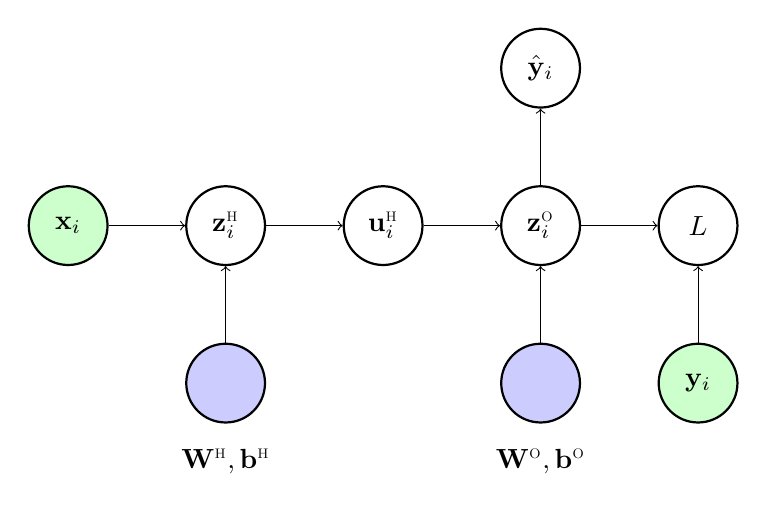
\begin{tikzpicture}[xscale=2,yscale=2,node distance=2cm]
    \tikzstyle{var}=[circle,thick,minimum size=1cm,draw]
    \tikzstyle{param}=[circle,thick,minimum size=1cm,draw,fill=blue!20]
    \tikzstyle{data}=[circle,thick,minimum size=1cm,draw,fill=green!20]

    \node(x)  [data] {$\xbf_i$};
    \node(zh) [var,right of=x] {$\zbf^\hid_i$};
    \node(uh) [var,right of=zh] {$\ubf^\hid_i$};
    \node(zo) [var,right of=uh] {$\zbf^\out_i$};
    \node(yh) [var,above of=zo] {$\hat{\ybf}_i$};
    \node(L)  [var,right of=zo] {$L$};
    \node(y)  [data,below of=L] {$\ybf_i$};

    \node(Wh) [param,below of=zh] {};
    \node  [below of=Wh,yshift=1cm] {$\Wbf^\hid,\bbf^\hid$};
    \node(Wo) [param,below of=zo] {};
    \node  [below of=Wo,yshift=1cm] {$\Wbf^\out,\bbf^\out$};

    \draw [->] (x) -- (zh);
    \draw [->] (zh) -- (uh);
    \draw [->] (uh) -- (zo);
    \draw [->] (zo) -- (yh);
    \draw [->] (zo) -- (L);
    \draw [->] (Wh) -- (zh);
    \draw [->] (Wo) -- (zo);
    \draw [->] (y) -- (L);

\end{tikzpicture}
\caption{Computation graph for the neural network mapping the the training data $(\xbf_i,y_i)$
and parameters to the loss function $L$.  Parameters are shown in light blue
and data in light green.}
\label{fig:compgraph}
\end{figure}

\item \emph{Back propagation:}
Once data is represented in a computation graph, we can compute
gradients of any of the output variables from the parameters
by a procedure called \emph{back propagation}.
Since we want to compute the gradient of the loss $L$, we start
at that node.  Then, we find the path going backwards in the
computation graph towards all the parameters to compute the gradients.
Note that the data $(\xbf_i,y_i)$ is fixed, so we don't take the gradients with respect to $\xbf_i$ or $\ybf_i$.  As we move backwards in the path,
we compute the gradients via chain rule.

For the computation graph in Fig.~\ref{fig:compgraph}, we could follow the following steps:
\begin{itemize}
\item $L \arr \zbf^\out$:  Compute the gradient $\partial L/\partial \zbf^\out$.

\item $\zbf^\out \arr \Wbf^\out, \bbf^\out, \ubf^\hid$: Compute the gradients:
\[
    \frac{\partial \zbf^\out}{\partial \Wbf^\out}, \quad
    \frac{\partial \zbf^\out}{\partial \bbf^\out}, \quad
    \frac{\partial \zbf^\out}{\partial \ubf^\hid}.
\]
Then apply chain rule to compute the gradient of $L$,
\begin{align*}
    \frac{\partial L}{\partial \Wbf^\out} &= \frac{\partial L}{\partial \zbf^\out} \cdot \frac{\partial \zbf^\out}{\partial \Wbf^\out}, \quad
    \frac{\partial L}{\partial \bbf^\out} = \frac{\partial L}{\partial \zbf^\out} \cdot \frac{\partial \zbf^\out}{\partial \bbf^\out}, \quad
    \frac{\partial L}{\partial \ubf^\hid} = \frac{\partial L}{\partial \zbf^\out} \cdot \frac{\partial \zbf^\out}{\partial \ubf^\hid},
\end{align*}
where the multiplication $\cdot$ represents a tensor dot-product.

\item $\ubf^\hid \arr \zbf^\hid$: Compute $\partial \ubf^\hid/\partial \zbf^\hid$ and then use chain rule
Then, we apply chain rule,
\[
    \frac{\partial L}{\partial \zbf^\hid} = \frac{\partial L}{\partial \ubf^\hid} \cdot \frac{\partial \ubf^\hid}{\partial \zbf^\hid}.
\]

\item $\zbf^\hid \arr \Wbf^\hid, \bbf^\hid$:
We have $\zbf^\hid_i = \Wbf^\hid \xbf_i+ \bbf^\hid$.  Compute the gradients:
\[
    \frac{\partial \zbf^\hid}{\partial \Wbf^\hid}, \quad
    \frac{\partial \zbf^\hid}{\partial \bbf^\hid}.
\]
Then apply chain rule to compute the gradient of $L$,
\begin{align*}
    \frac{\partial L}{\partial \Wbf^\hid} &= \frac{\partial L}{\partial \zbf^\hid} \cdot \frac{\partial \zbf^\hid}{\partial \Wbf^\hid}, \quad
    \frac{\partial L}{\partial \bbf^\hid} = \frac{\partial L}{\partial \zbf^\hid} \cdot \frac{\partial \zbf^\hid}{\partial \bbf^\hid}.
\end{align*}
\end{itemize}
We illustrate the details in the problems below.
\end{itemize}


\paragraph*{Problems}
\begin{enumerate}
\item Consider a neural network \eqref{eq:nn} acting on
a mini-batch of training samples $(\xbf_i,y_i)$, $i=1,\ldots,N$.  Suppose that $y_i \in \{1,\ldots,K\}$ so that the problem
is $K$-class classification, we use the categorial cross-entropy loss \eqref{eq:gloss_mc} and a ReLU activation.
Derive the back-propagation equations for all steps.

\item \label{prob:cg_exp}
Suppose that we are given a mini-batch of training data $(\xbf_i,y_i)$, $i=1,\ldots,N$, 
and we try to fit a model to the data of the form,
\begin{align*}
    \zbf_i    &= \Wbf\xbf_i + \bbf, \quad
    \hat{y}_i = \sum_{j=1}^M \alpha_j\exp(z_{ij}),
\end{align*}
for unknown parameters $\theta=(\Wbf,\bbf,\alpha)$.  Here $M$ is the dimension
of the hidden variables $\zbf_i$.  We use the squared error loss function,
\[
    L = \sum_{i=1}^N L_i, \quad L_i = (y_i-\hat{y}_i)^2.
\]
\begin{enumerate}[(a)]
\item Add an intermediate variable $\ubf_i = \exp(\zbf_i)$, by which we mean
$u_{ij} = \exp(z_{ij})$.  Draw the computation graph showing the mapping
from the inputs $\xbf_i$ and the parameters $\theta$ to the loss function, $L$.
Also, write the equations for each step in the computation graph.

\item Write the back-propagation equations to obtain the 
gradients with respect to the parameters $\theta$.
\end{enumerate}


\end{enumerate}

\paragraph*{Solutions}
\begin{enumerate}
\item  We work our way backward starting at $L$ along paths to get to the parameters:
\begin{itemize}
\item $L \arr \zbf^\out$:  The loss function is the categorial cross-entropy \eqref{eq:gloss_mc}.
Therefore, the gradient components are
\[
    \frac{\partial L}{\partial z^\out_{ij}} = \frac{\partial g_{\rm loss}(\zbf^\out_i,y_i)}{\partial z^\out_{ij}}
    = \frac{e^{z^\out_{ij}}}{\sum_{\ell=1}^K e^{z^\out_{i\ell}}} -  r_{ij}.
\]

\item $\zbf^\out \arr \Wbf^\out, \bbf^\out, \ubf^\hid$:
We have $\zbf^\out_i = \Wbf^\out \ubf^\hid_i + \bbf^\out$.  Therefore,
\[
    z^\out_{ij} = \sum_k W^\out_{jk}u^\hid_{ik} + b^\out_j.
\]
Hence, we have the derivatives,
\[
    \frac{\partial z^\out_{ij}}{\partial W^\out_{jk}} = u^\hid_{ik}, \quad
    \frac{\partial z^\out_{ij}}{\partial b^\out_{j}} = 1, \quad
    \frac{\partial z^\out_{ij}}{\partial u^\hid_{ik}} = W_{jk}.
\]
Using chain rule,
\begin{align*}
    \frac{\partial L}{\partial W^\out_{jk}} &= \sum_{i=1}^N \frac{\partial L}{\partial z^\out_{ik}}\frac{\partial z^\out_{ij}}{\partial W^\out_{jk}}
        = \sum_{i=1}^N \frac{\partial L}{\partial z^\out_{ik}}u^\hid_{ik}, \\
    \frac{\partial L}{\partial b^\out_{j}} &= \sum_{i=1}^N \frac{\partial L}{\partial z^\out_{ik}}\frac{\partial z^\out_{ij}}{\partial b^\out_{j}}
        = \sum_{i=1}^N \frac{\partial L}{\partial z^\out_{ik}}, \\
    \frac{\partial L}{\partial u^\hid_{ik}} &= \sum_{j=1}^{N_o} \frac{\partial L}{\partial z^\out_{ij}}\frac{\partial z^\out_{ij}}{\partial u^\hid_{ik}}
        \sum_{j=1}^{N_o} \frac{\partial L}{\partial z^\out_{ij}}W_{jk}.
\end{align*}

\item $\ubf^\hid \arr \zbf^\hid$: We have
\[
    u^\hid_{ij} = g_{\rm act}(z^\hid_{ij}) = \max(0, z^\hid_{ij}).
\]
Hence,
\[
    \frac{\partial u^\hid_{ij}}{\partial z^\hid_{ij}} = \begin{cases}
        1, & \mbox{if } z^\hid_{ij} > 0 \\
        0, & \mbox{if } z^\hid_{ij} < 0.
    \end{cases}.
\]
Then, we apply chain rule,
\[
    \frac{\partial L}{\partial z^\hid_{ij}}  = \frac{\partial L}{\partial u^\hid_{ij}}\frac{\partial u^\hid_{ij}}{\partial z^\hid_{ij}}.
\]

\item $\zbf^\hid \arr \Wbf^\hid, \bbf^\hid$:
We have $\zbf^\hid_i = \Wbf^\hid \xbf_i+ \bbf^\hid$.  Therefore,
\[
    z^\hid_{ij} = \sum_k W^\hid_{jk}x_{ik} + b^\hid_j.
\]
Hence, we have the derivatives,
\[
    \frac{\partial z^\hid_{ij}}{\partial W^\hid_{jk}} = x_{ik}, \quad
    \frac{\partial z^\hid_{ij}}{\partial b^\hid_{j}} = 1.
\]
Using chain rule,
\begin{align*}
    \frac{\partial L}{\partial W^\hid_{jk}} &= \sum_{i=1}^N \frac{\partial L}{\partial z^\hid_{ik}}\frac{\partial z^\hid_{ij}}{\partial W^\hid_{jk}}
        = \sum_{i=1}^N \frac{\partial L}{\partial z^\hid_{ik}}x_{ik}, \\
    \frac{\partial L}{\partial b^\hid_{jk}} &= \sum_{i=1}^N \frac{\partial L}{\partial z^\hid_{ik}}\frac{\partial z^\hid_{ij}}{\partial b^\hid_{j}}
        = \sum_{i=1}^N \frac{\partial L}{\partial z^\hid_{ik}}.        
\end{align*}

\end{itemize}


\begin{figure}
\center
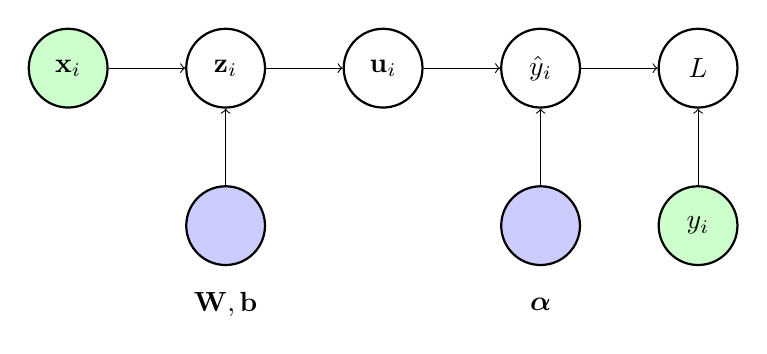
\begin{tikzpicture}[xscale=2,yscale=2,node distance=2cm]
    \tikzstyle{var}=[circle,thick,minimum size=1cm,draw]
    \tikzstyle{param}=[circle,thick,minimum size=1cm,draw,fill=blue!20]
    \tikzstyle{data}=[circle,thick,minimum size=1cm,draw,fill=green!20]

    \node(x)  [data] {$\xbf_i$};
    \node(z) [var,right of=x] {$\zbf_i$};
    \node(u) [var,right of=z] {$\ubf_i$};
    \node(yh) [var,right of=u] {$\hat{y}_i$};
    \node(L)  [var,right of=yh] {$L$};
    \node(y)  [data,below of=L] {$y_i$};

    \node(W) [param,below of=z] {};
    \node  [below of=W,yshift=1cm] {$\Wbf,\bbf$};
    \node(alpha) [param,below of=yh] {};
    \node  [below of=alpha,yshift=1cm] {$\alphabf$};

    \draw [->] (x) -- (z);
    \draw [->] (W) -- (z);
    \draw [->] (z) -- (u);
    \draw [->] (alpha) -- (yh);
    \draw [->] (u) -- (yh);
    \draw [->] (yh) -- (L);
    \draw [->] (y) -- (L);

\end{tikzpicture}
\caption{Computation graph for Problem~\ref{prob:cg_exp}
mapping the the training data $(\xbf_i,y_i)$
and parameters to the loss function $L$.  Parameters are shown in light blue
and data in light green.}
\label{fig:compgraph_exp}
\end{figure}

\item

\begin{enumerate}[(a)]
\item If we substitute $\ubf_i = \exp(\zbf_i)$ we can write the mapping from
the set of $\xbf_i$'s to $L$ as
\begin{align*}
    \zbf_i    &= \Wbf\xbf_i + \bbf \\
    \ubf_i &= \exp(\zbf_i), \quad \hat{y}_i = \alphabf\tran \ubf_i \\
    L &= \sum_{i=1}^N (y_i-\hat{y}_i)^2.
\end{align*}
The computation graph is shown in Fig.~\ref{fig:compgraph_exp}.

\item We perform back-propagation in the following steps:
\begin{itemize}
\item $L \arr \hat{\ybf}$:  The components of the gradient are:
\[
    \frac{\partial L}{\partial \hat{y}_i} = 2(\hat{y}_i - y_i).
\]

\item $\hat{\ybf} \arr \alphabf, \ubf$:  We have
\[
    \hat{y}_i = \alphabf\tran \ubf_i = \sum_{j=1}^M \alpha_ju_{ij} \Rightarrow
    \frac{\partial \hat{y}_i}{\partial u_{ij}}.
\]
Therefore,
\[
    \frac{\partial \hat{y}_i}{\partial u_{ij}} = \alpha_j, \quad 
    \frac{\partial \hat{y}_i}{\partial \alpha_j} = u_{ij}.
\]
Applying chain rule,
\begin{align*}
    \frac{\partial L}{\partial \alpha_j} &= \sum_{i=1}^N 
    \frac{\partial L}{\partial \hat{y}_i}\frac{\partial \hat{y}_i}{\partial \alpha_j}
    = \sum_{i=1}^N  \frac{\partial L}{\partial \hat{y}_i}u_{ij} \\
    \frac{\partial L}{\partial u_{ij}} &= 
    \frac{\partial L}{\partial \hat{y}_i}\frac{\partial \hat{y}_i}{\partial u_{ij}}
    = \sum_{i=1}^N  \frac{\partial L}{\partial \hat{y}_i}\alpha_j.
\end{align*}

\item $\ubf \arr \zbf$: Since $u_{ij} = \exp(z_{ij})$, we have the derivative,
\[
    \frac{\partial u_{ij}}{\partial z_{ij}} = \exp(z_{ij}).
\]
Using chain rule:
\[
    \frac{\partial L}{\partial z_{ij}} = \frac{\partial L}{\partial u_{ij}}\frac{\partial u_{ij}}{\partial z_{ij}}
    = \frac{\partial L}{\partial u_{ij}}\exp(z_{ij}).
\]

\item $\zbf \arr \Wbf,\bbf$:  Since $\zbf_i = \Wbf\xbf_i + \bbf$, 
Therefore,
\[
    z_{ij} = \sum_k W_{jk}x_{ik} + b_j.
\]
Hence, we have the derivatives,
\[
    \frac{\partial z_{ij}}{\partial W_{jk}} = u_{ik}, \quad
    \frac{\partial z_{ij}}{\partial b_{j}} = 1.
\]
Applying chain rule,
\begin{align*}
    \frac{\partial L}{\partial W_{jk}} &= 
        \sum_i \frac{\partial L}{\partial z_{ij}}\frac{\partial z_{ij}}{\partial W_{jk}} 
        = \sum_i \frac{\partial L}{\partial z_{ij}}u_{ik}, \\
    \frac{\partial L}{\partial b_{j}} &=
        \sum_i \frac{\partial L}{\partial z_{ij}}\frac{\partial z_{ij}}{\partial b_{j}}
        = \sum_i \frac{\partial L}{\partial z_{ij}}. 
\end{align*}

\end{itemize}

\end{enumerate}



\end{enumerate}

\end{document}


